\documentclass{article}

\usepackage{graphicx} % for images
\usepackage{amsmath} % for math
\usepackage{amssymb} % for \mathbb
\usepackage{siunitx} % for \SI, \num
\usepackage{hyperref} % for \url{}

% This stuff is for figures
\usepackage{float}
\DeclareGraphicsExtensions{.pdf, .png, .jpg}

% coloring of links for PDF format
\hypersetup{
    colorlinks=true,
    urlcolor=blue,
    linkcolor=black
}

% \c command redefinition (for monospaced font)
\renewcommand{\c}[1]{\texttt{#1}}
% \today command re-definition
%https://tex.stackexchange.com/questions/112932/today-month-as-text
\renewcommand{\today}{\ifnum\number\day<10 0\fi \number\day \space%
\ifcase \month \or January\or February\or March\or April\or May%
\or June\or July\or August\or September\or October\or November\or December\fi\space%
\number \year} 

\begin{document}
\begin{titlepage}
	\centering
	
\includegraphics[width=0.25\textwidth]{Images/247px-CSU-Longbeach_seal}\par\vspace{1cm}
	{\scshape\Large California State University, Long Beach \par}
	\vspace{1cm}
	{\scshape\Large CECS 447\par}
	\vspace{1.5cm}
	{\huge\bfseries Project 4\par}
	\vspace{2cm}
    {\Large\itshape Rodrigo Becerril Ferreyra\par}
    {\itshape\Large Student ID 017584071 \par}
	\vfill
    A project that demonstrates the ST7735
	Color LCD.

	\vfill

% Bottom of the page
	{\large \today\par}
\end{titlepage}

\section{Introduction}
The purpose of this project is to demonstrate some of the
capabilities of the ST7735 Color LCD. The display is
128x160 square pixels, and is capable of displaying
16-bit color (16 bits total divided among the three color
channels). For the project, my objectives were to create a
scene that includes all of the following:
\begin{itemize}
	\item a background with two different colors.
	\item a circle, a vertical line, a horizontal line,
	and a diagonal line.
	\item a moving object.
	\item at least one line of text with different sizes
	and different colors.
\end{itemize}

My theme is based on the video game series \emph{Portal},
in which the player uses a ``portal gun'' in order to create
portals to teleport around the ``test areas'' and solve
puzzles. If the player places a portal on the ceiling,
and the complementary portal on the floor just below,
the player's character will fall through the portal
on the floor and come out from the portal on the ceiling.
This will repeat indefinitely (as long as the player
doesn't move), and the player's character will continue to
speed up until reaching terminal velocity. An example of
this behavior can be found here (image Copyright (C)
Valve, used under fair use for education):
\url{https://i.kym-cdn.com/photos/images/original/000/192/001/tumblr_lt2crpCRxY1r2yv3qo1_500.gif}.

\section{Operation}
The program works by using the provided Adafruit libraries
to interface with the ST7735 LCD. It calls several functions,
mostly \c{ST7735\_DrawCircle()} and \c{ST7735\_DrawLine()};
this is because these are used for drawing the stick figure.

The program animates the stick figure by repeatedly drawing
it in white, waiting a while, then drawing it again in black.
Because the color of the background is also black, this
creates the illusion of the stick figure being erased
or deleted. The delay is implemented using the SysTick
hardware timer.

A video of the embedded system in operation can be found
here: \url{https://youtu.be/8JxxkUPIeaU}.

\section{Theory}
There is not much theory to this project; it is simply
utilizing the Adafruit libraries to create an animation.

\section{Hardware Design}
Figure \ref{schematic} shows the connections for my
specific version of the ST7735 LCD. Note that there are
more pins that are not shown; any pin not shown is not
connected (floating).

\begin{figure}[H]
	\centering
	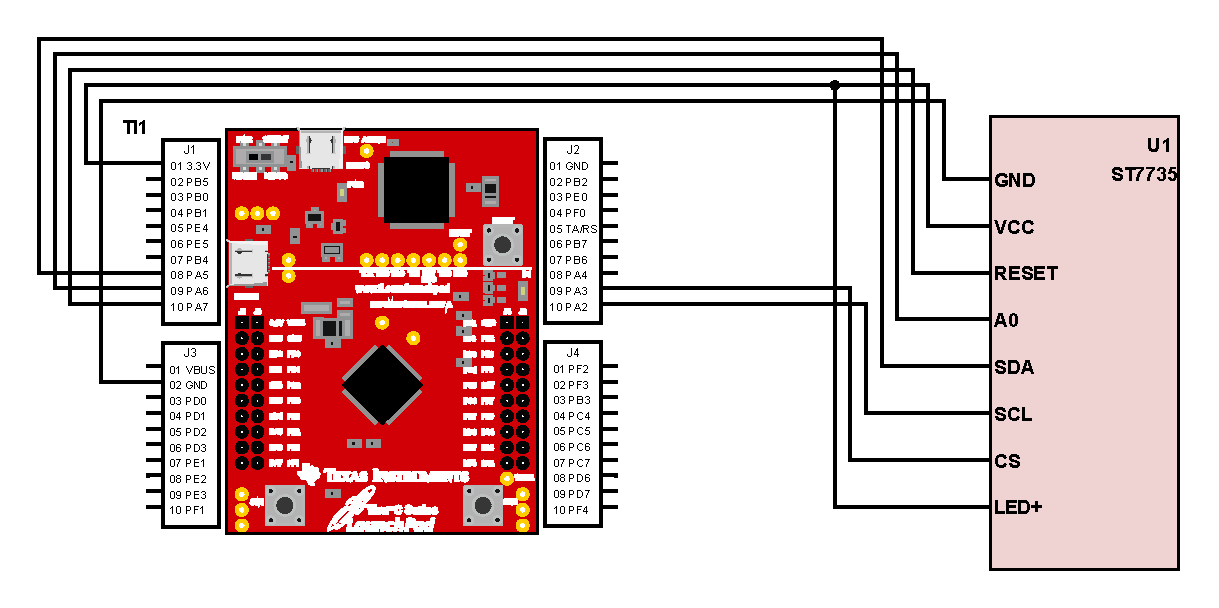
\includegraphics[width=\textwidth]{Images/schemeit-project}
	\caption{The pin connections for my version of the
	ST7735 LCD.}
	\label{schematic}
\end{figure}

\begin{figure}[H]
	\centering
	\includegraphics[width=\textwidth]{"Images/20211204_172654"}
	\caption{An image of the embedded system in action.}
	\label{image}
\end{figure}

\section{Software Design}
Most of the work was already done for us courtesy of
Adafruit, as we are using their libraries to communicate
to the LCD. My contribution was simply the \c{main()}
function. The following is a breakdown of what the
\c{main()} function does:
\begin{enumerate}
	\item First, the program draws the background. It
	consists of a mostly black screen. There is a white
	section on the top, which is where all of the text
	goes.
	\item Next, the program draws the text. First, some
	simple text with a size of 1 is drawn in black using
	the function \c{ST7735\_DrawString()}. Next, some
	more advanced text in different size and colors is
	drawn by invoking the \c{ST7735\_DrawCharS()} function
	in a \c{for} loop.
	\item Finally, the program enters an infinite loop.
	This loop repeatedly draws and erases a stick figure
	in various positions on the screen in order to
	simulate falling.
\end{enumerate}

The main challenge I faced while writing the program is
sometimes having to draw the stick figure
in parts, for example having its head on the ground
but its body on the ceiling. This made it much harder
to use a function for drawing the person like in the
example given to us. It definitely is not impossible, but
for a project of this scale, I don't think it was necessary.

After every iteration of the stick figure is drawn, the same
exact commands are used to erase the figure. This is done
by drawing the figure in black instead of white.

\section{Conclusion}
This project was relatively simple compared to some
previous projects. All that was really required was some
creativity and knowing how to use the library that was
given to us. Overall, this project was quite enjoyable
and informative.

\end{document}
